\documentclass[a4paper,11pt]{article}
\usepackage[colorlinks=true,linkcolor=blue,allcolors=red]{hyperref}

\renewcommand\thefootnote{\textcolor{red}{\arabic{footnote}}}

\title{\LARGE \bf 
    Nonfunctional Requirements
}
\author{\\\\ Cristian Camilo Serna Betancur \\\\ Andres Grisales Gonzalez  
\\\\ John Fredy Mejia Serna}

\begin{document}
\maketitle
\tableofcontents

\section{A}
\section{B}
\section{C}
\section{D}
\section{E}
\section{Desacoplamiento}
Cuando hablamos de Acoplamiento nos referimos a la relación entre dos entidades en un sistema de software (generalmente clases).
Cuando una clase usa otra clase, o se comunica con ella, se dice que 'depende' de esa otra clase, por lo que estas clases están
'acopladas'. Al menos uno de ellos 'sabe' sobre el otro. La idea es que deberíamos tratar de mantener el acoplamiento entre clases
en nuestros sistemas lo más 'flojo' posible: de ahí 'acoplamiento suelto' o, a veces 'desacoplamiento'. De esta forma, una de las
tantas maneras para evitar este acoplamiento, es el uso de interfaces.

\section{Sustituibilidad}
Buscamos la capacidad de substitución correcta de subtipos de una clase, la forma de tener una sustituibilidad
adecuada es respetando correctamente el Principio de substitución de Liskov.

\section{Aciclicidad}
Con la aciclicidad buscamos evitar dependencias cíclicas entre clases y entre paquetes, es una muy buena métrica para medir la mantenibilidad 
del software, cuando nos encontremos con dependencias cíclicas debemos sentarnos un rato y pensar como modificamos ya sea la 
ubicación de clases dentro paquetes de manera que podamos romper esa ciclicidad que es dañina.

Por ejemplo, así no:
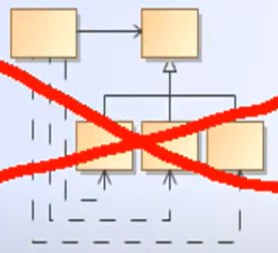
\includegraphics{assets/cicl.PNG}
Así tampoco:
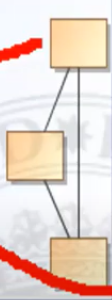
\includegraphics{assets/cicl2.PNG}
Así sí:
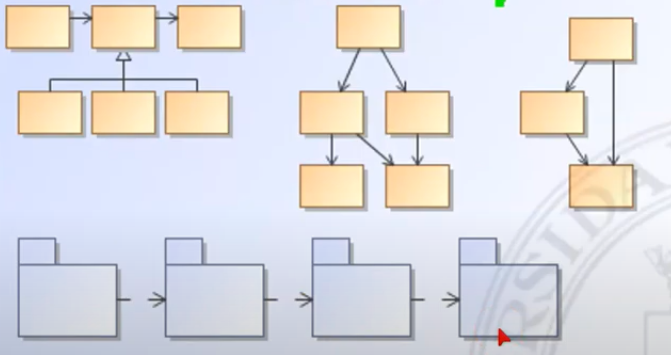
\includegraphics{assets/good cicl.PNG}
\end{document}
